\newpage
\section{Test of the Equalizer}
In this part, all the requirements related to the equalizer will be tested if they are fulfilled. 


\subsection{Test of \autoref{req:equalizer}}
According to \autoref{req:equalizer}, the gain value in each individual filter must be changeable by the user. This requirement has not been completely fulfilled since there has not been made an actual user interface for the effect. It is possible to change the gain of each individual filter, but only by writing it directly in the program. A test was made to prove this, where the peak filters with $\omega_0 =$ \SI{200}{\hertz} and $\omega_0 =$ \SI{3200}{\hertz} is set to amplify respectively \SI{6}{\decibel} and \SI{12}{\decibel}. 
\autoref{fig:tests:eq_gain} show the result of the test.

\begin{figure}[htbp!]
    \centering
        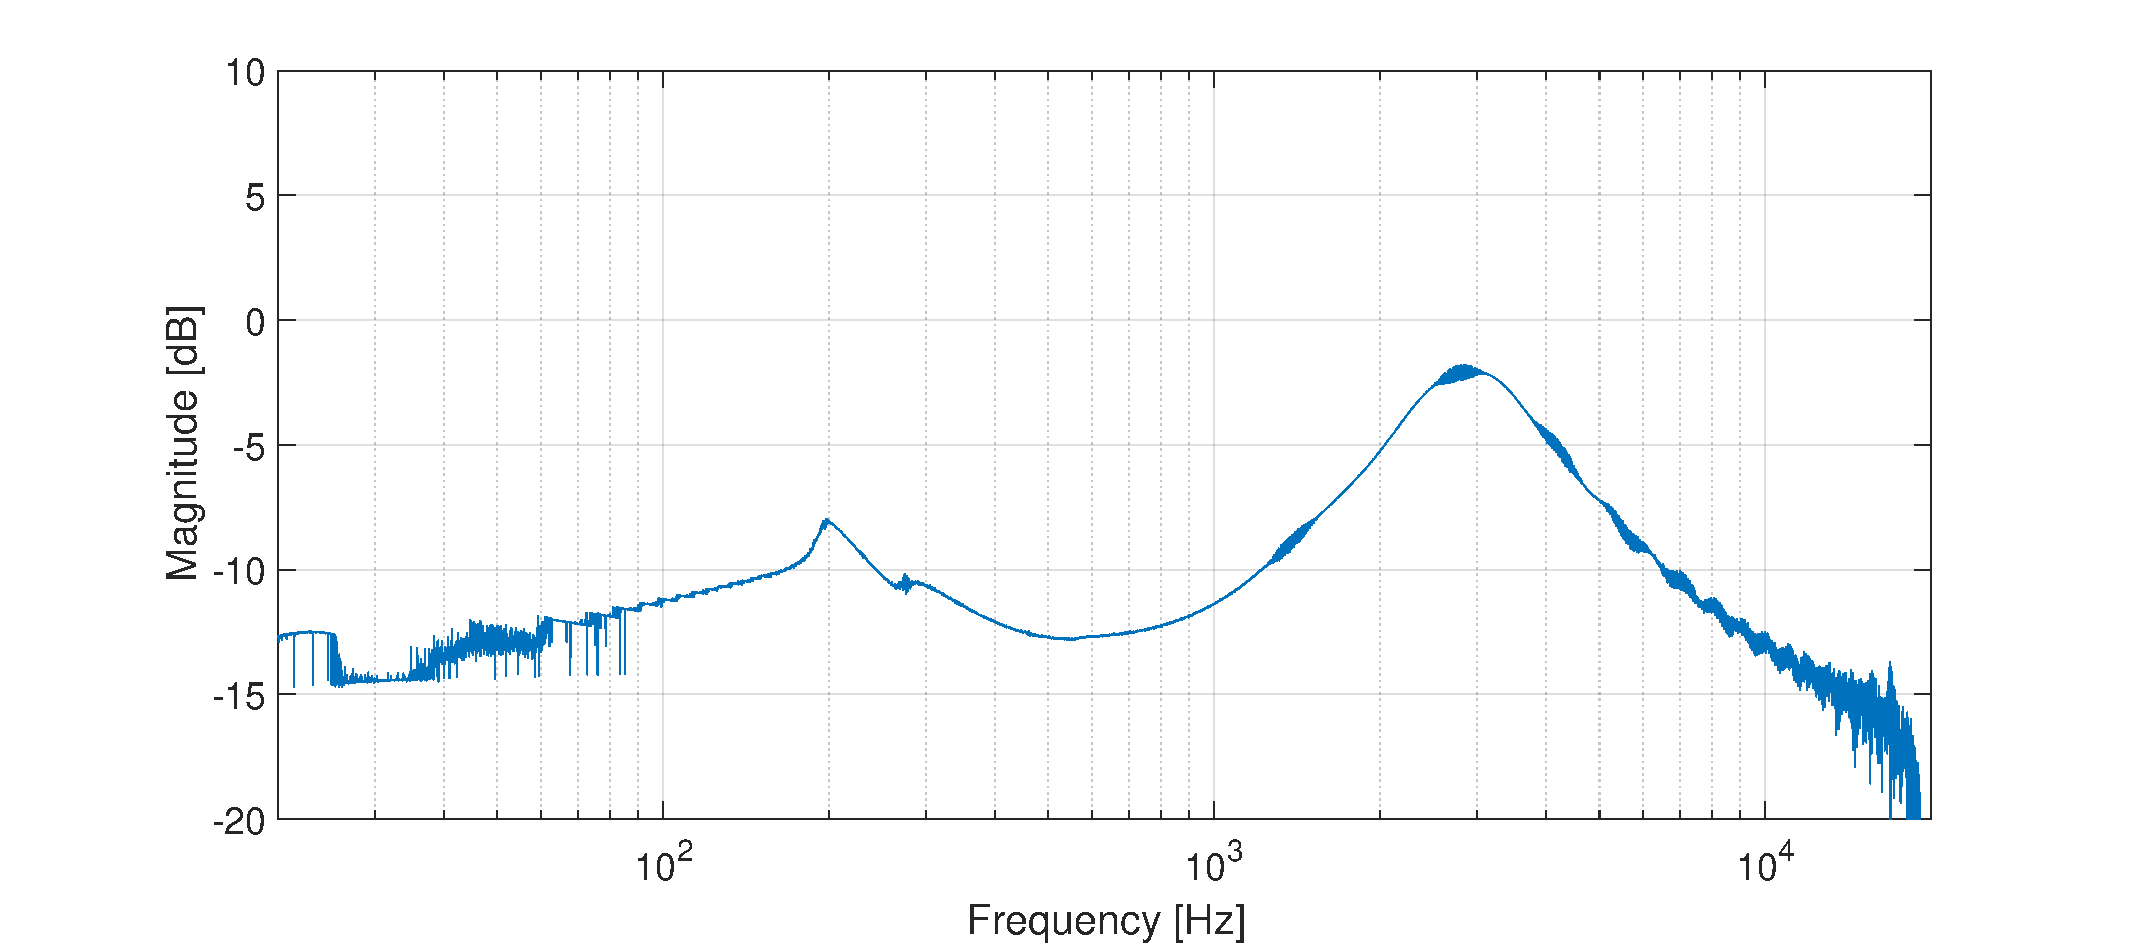
\includegraphics[width=\textwidth]{eq_200Hz_6db_3200Hz_12db.pdf}
        \caption{Measurement of the equalizer, where the peak filters with $\omega_0 =$ \SI{200}{\hertz} and $\omega_0 =$ \SI{3200}{\hertz} is set to amplify respectively \SI{6}{\decibel} and \SI{12}{\decibel}.}
        \label{fig:tests:eq_gain}
  \end{figure}



\subsection{Test of \autoref{req:equalizer2}}
According to \autoref{req:equalizer2}, each individual band must, when fully amplified, drop \SI{6}{\decibel} at the neighbouring center frequencies. A test was made using  the setup in \autoref{chap:effect_test_response}, where all the individual, fully amplified, filters and the combined filter, with all filters fully amplified, were tested. \autoref{fig:tests:eq_filters} shows the result of the test, where the upper blue graph is the combined equalizer and the others are the individual filters.

\begin{figure}[htbp!]
    \centering
        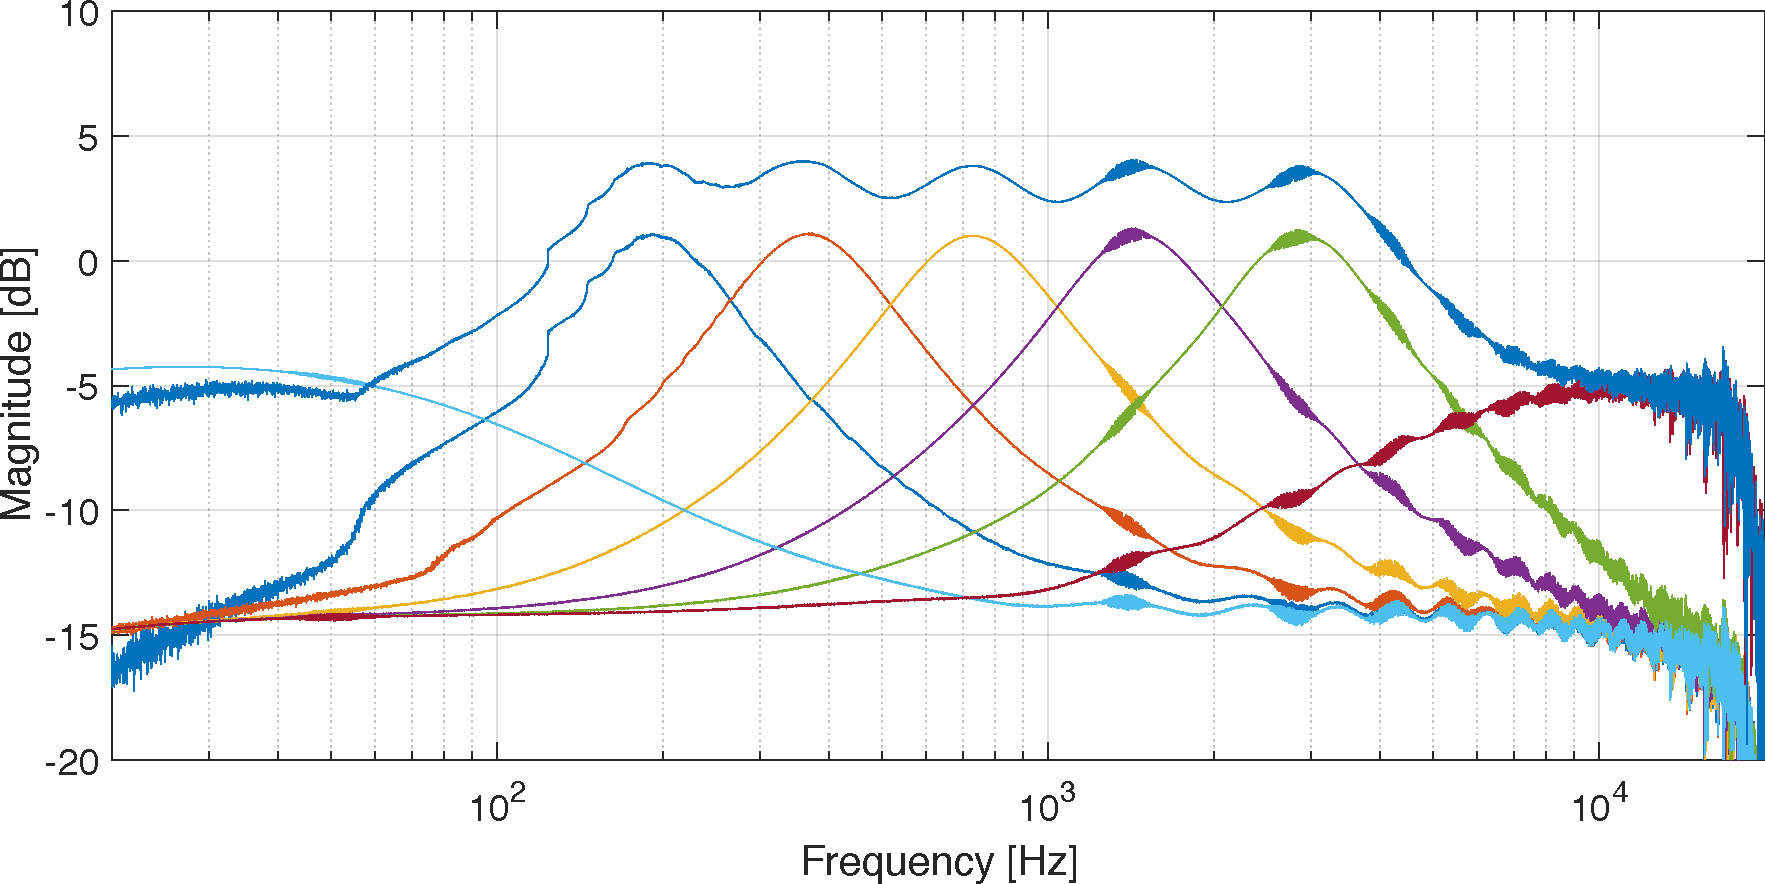
\includegraphics[width=\textwidth]{tested_eq.pdf}
        \caption{Measurement of the individual filters in the equalizer and the combined filter.}
        \label{fig:tests:eq_filters}
  \end{figure}
  
 In \autoref{fig:tests:eq_filters} it is seen that e.g. the peak filter with $\omega_0 =$ \SI{800}{\hertz} has dropped approximately \SI{6.5}{\decibel} at \SI{400}{\hertz} and \SI{1600}{\hertz}. It is also seen that at some frequencies, especially the high frequencies, the frequency response seems to oscillate. A measurement of the \gls{dsp}'s frequency response was made to investigate this. The result of the test i seen in \autoref{fig:tests:direct_dsp_gain}.

\begin{figure}[htbp!]
    \centering
        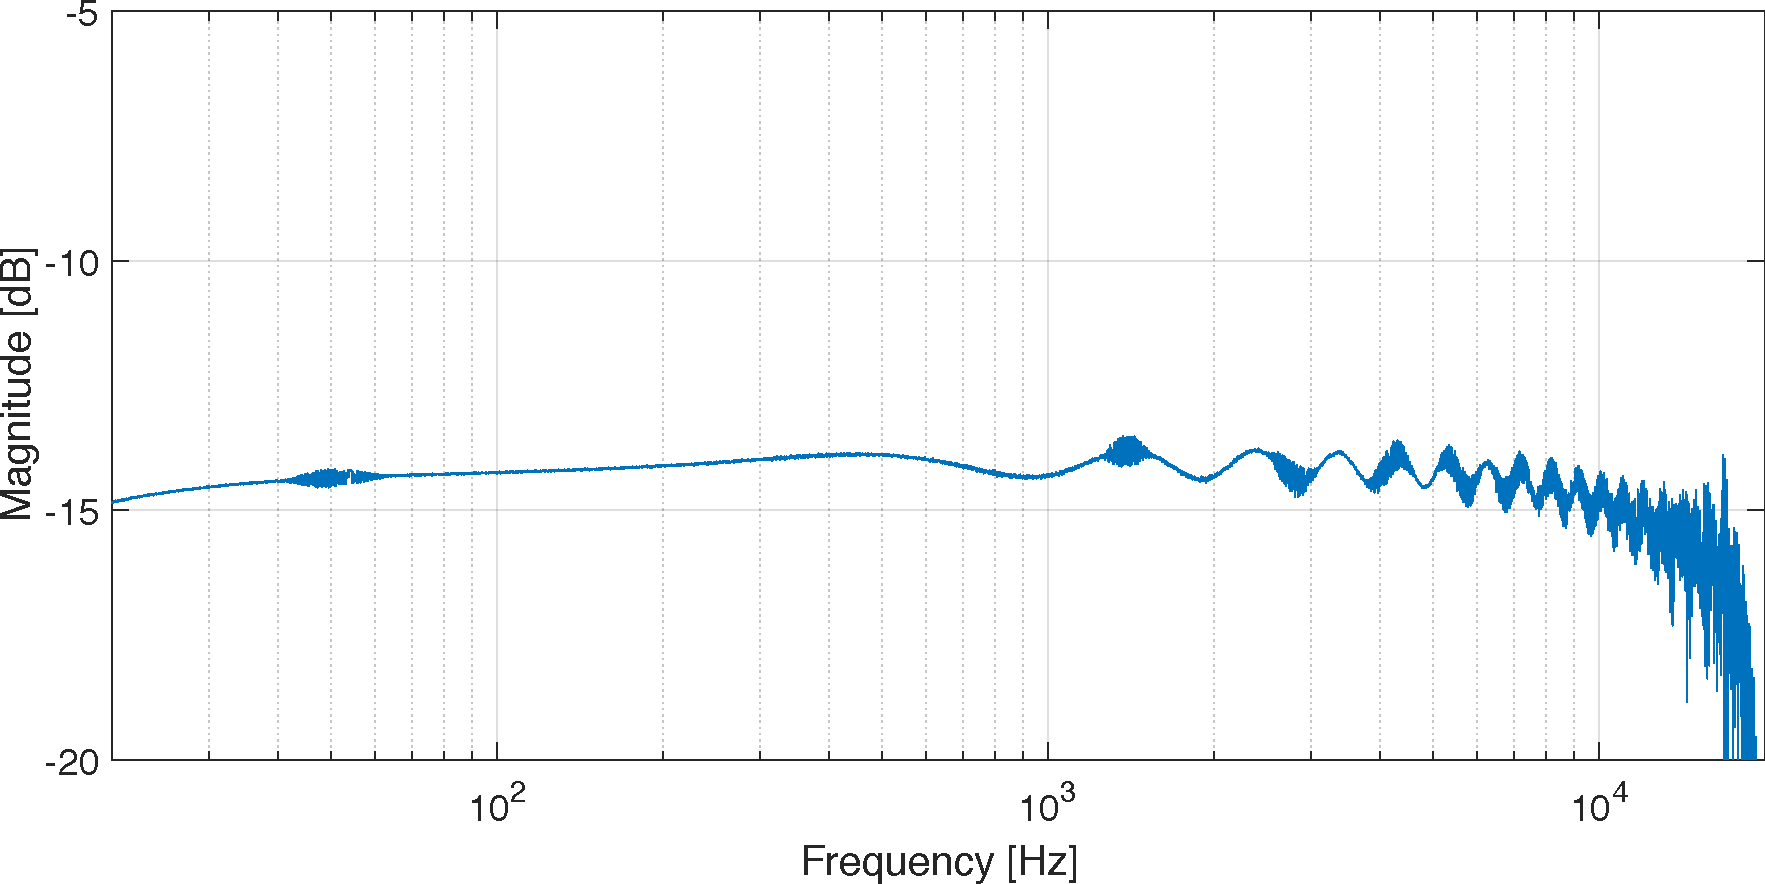
\includegraphics[width=\textwidth]{direct_dsp_gain.pdf}
        \caption{Measurement of the \gls{dsp}'s frequency response}
        \label{fig:tests:direct_dsp_gain}
  \end{figure}

\autoref{fig:tests:direct_dsp_gain} shows that the oscillations in \autoref{fig:tests:eq_filters} is because of the frequency response of the \gls{dsp}.
Thus the requirement is fulfilled. 

\subsection{Test Review of the Requirements for the Equalizer}
In \autoref{tab:test_of_eq_table} the conclusion for the requirements related to the equalizer is summed.

\begin{table}[H]
\centering
\caption{Recap of the requirements fulfilments for the equalizer test}
\label{tab:test_of_eq_table}
\begin{tabular}{|l|l|}
\hline
\rowcolor[HTML]{9B9B9B} 
\textbf{Requirement} & \textbf{Fulfilment State} \\ \hline
\textbf{\ref{req:equalizer}}    & \cmark *                     \\ \hline
\textbf{\ref{req:equalizer2}}    & \cmark                      \\ \hline

\end{tabular}
\end{table}




